\chapter{Evaluation}
\section{Vergleich zwischen alter und neuer Webseite}
Insgesamt haben sich die Graphen der alten Webseite durch den Einsatz von Data-Storytelling deutlich verändert. Bereits im Laufe der Arbeit wurden einige Beispiele von den alten Graphen ohne Data-Storytelling gezeigt. Dabei hat sich besonders der Graph zur Darstellung der kumulierten Schädigung von allen gemessenen Durchfahrten verändert. Die Schwierigkeit bei diesem Graphen ist die Menge an Daten, die dargestellt werden sollen. Dadurch ist es besonders auf der alten Webseite schwierig, auf einen Blick zu erkennen, welche Daten  relevant sind. Durch den Einsatz des Data-Storytellings konnten die Reize, die auf den Benutzer wirken, reduziert und die wichtigen Punkte des Graphen hervorgehoben werden. In der folgenden direkten Gegenüberstellung in Abbildung \ref{fig:schädigung_vergleich} ist die Verbesserung, trotz verschiedener Daten, gut zu erkennen.\\
\begin{figure}[!h]
    \centering
    \includegraphics[width=1\linewidth]{gfx/schädigung_davor.png}
    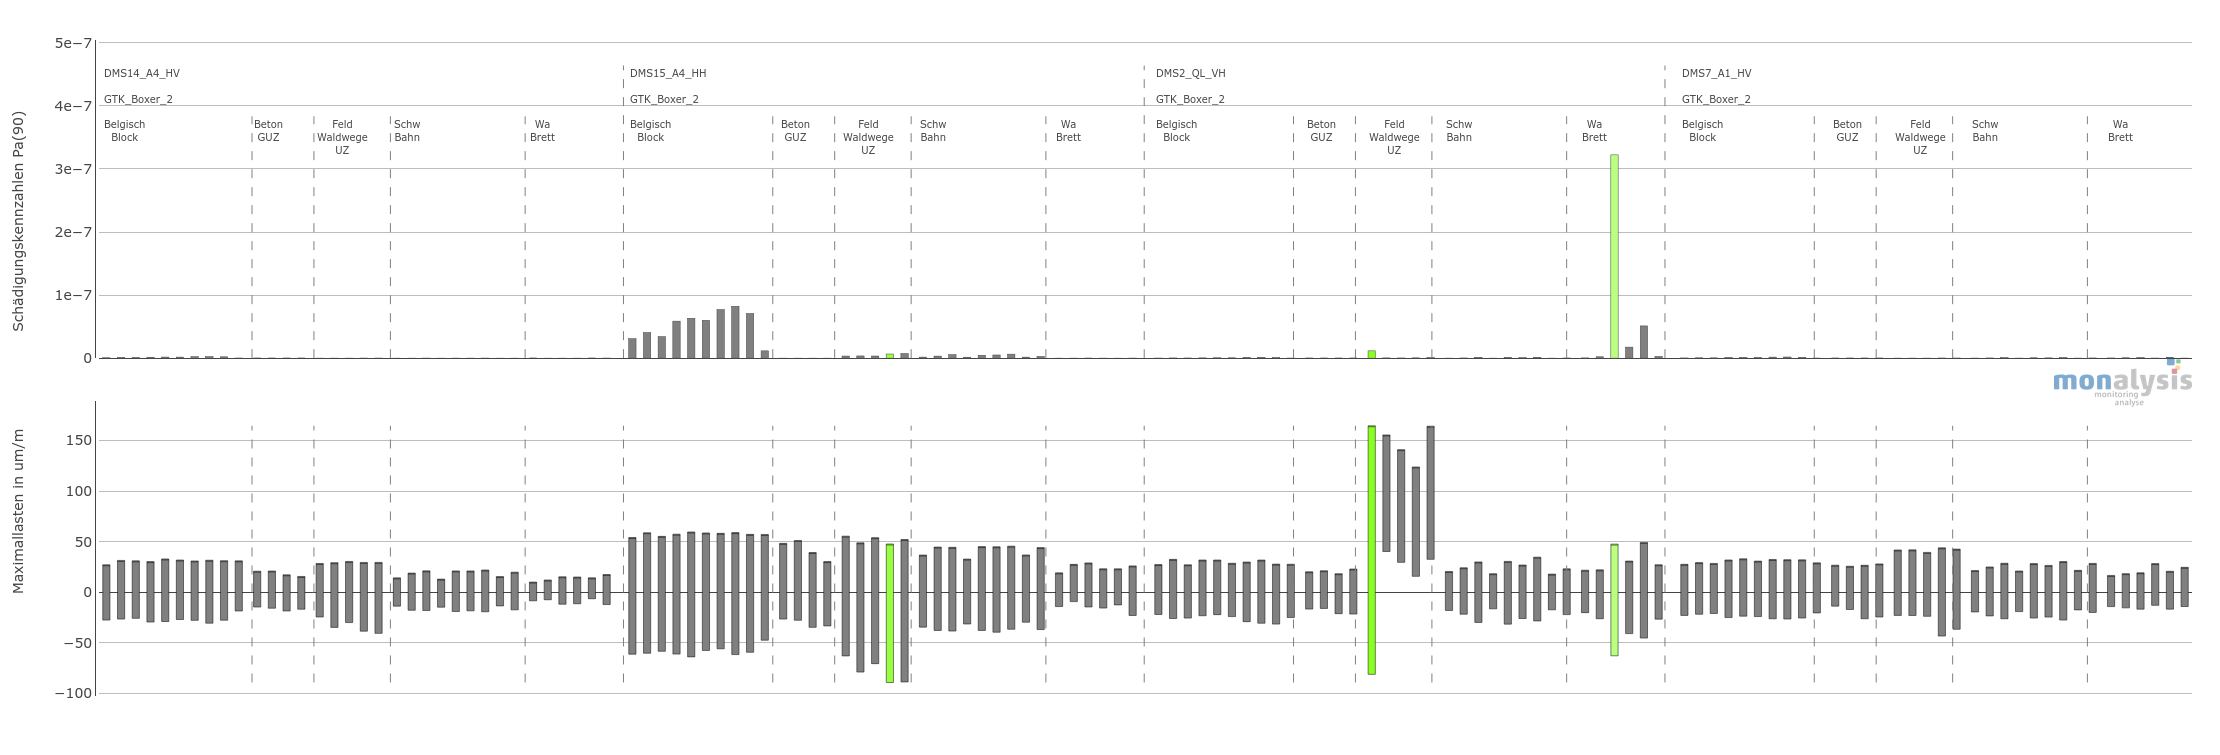
\includegraphics[width=1\linewidth]{gfx/new_schaedigung.png}
    \caption{Graph mit der kumulierten Schädigung im Vergleich}
    \label{fig:schädigung_vergleich}
\end{figure}
\noindent
Insbesondere bei Aktivierung des Top-Filters kann durch das Data-Storytelling schneller erkannt werden, welche Daten wie beschaffen sind \ref{fig:top_filter_vergleich}. 
\begin{figure}
    \centering
    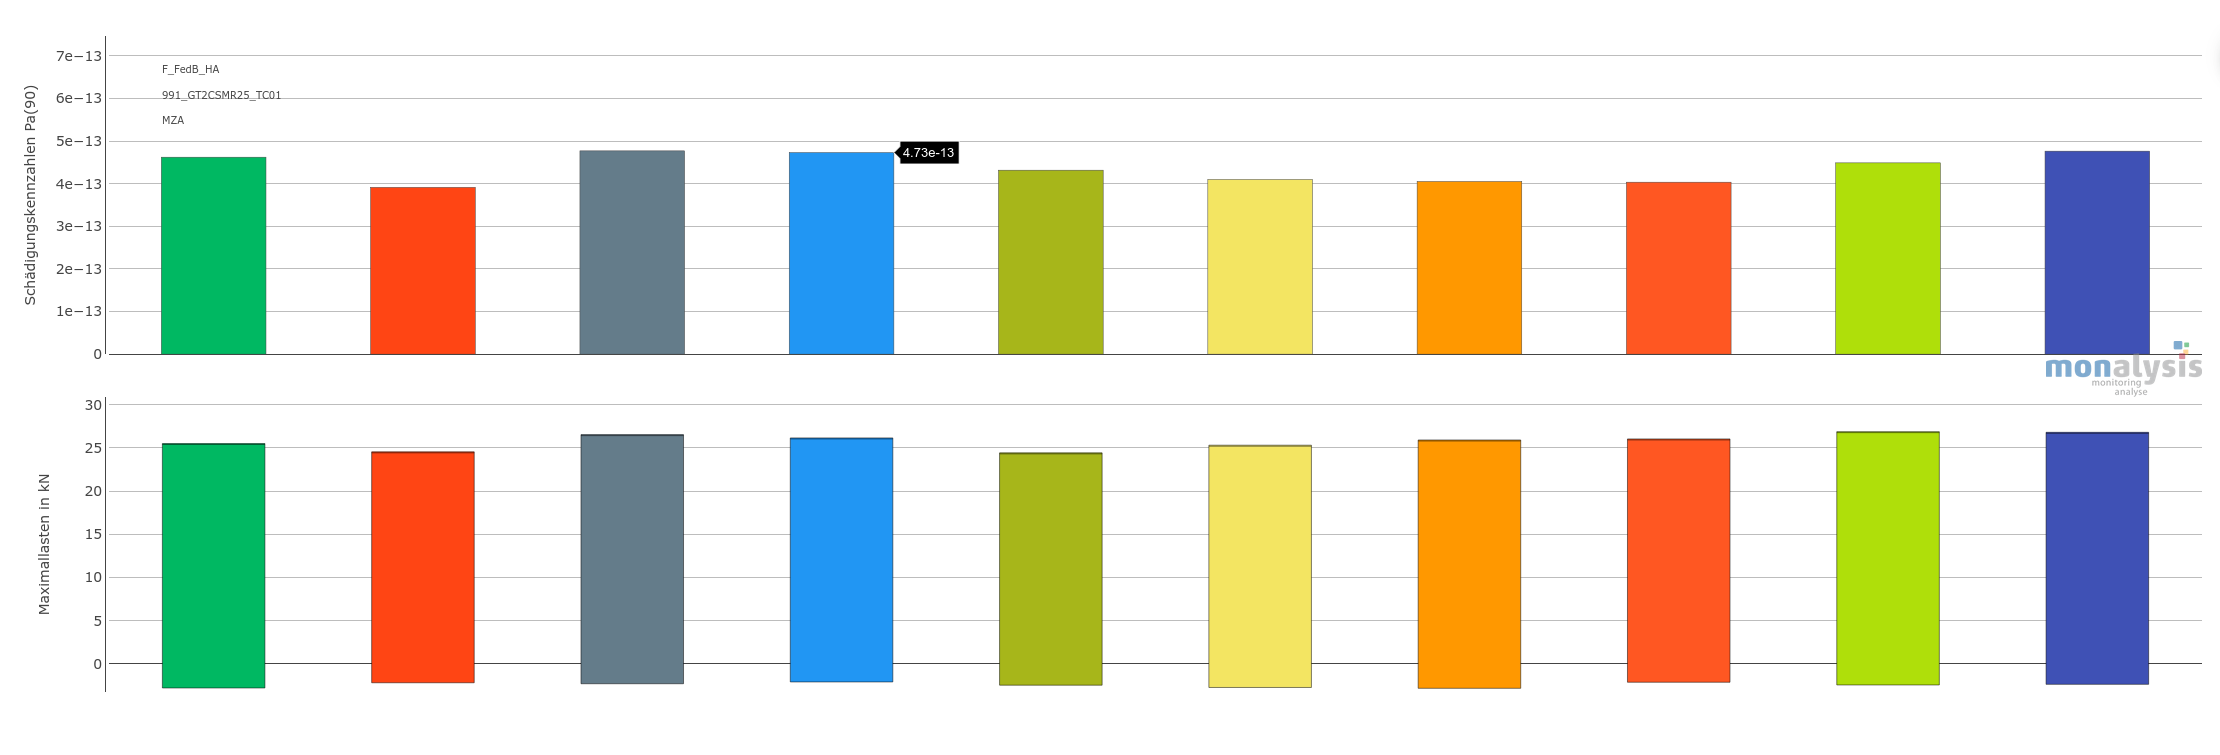
\includegraphics[width=1\linewidth]{gfx/top_vergleich_alt.png}
    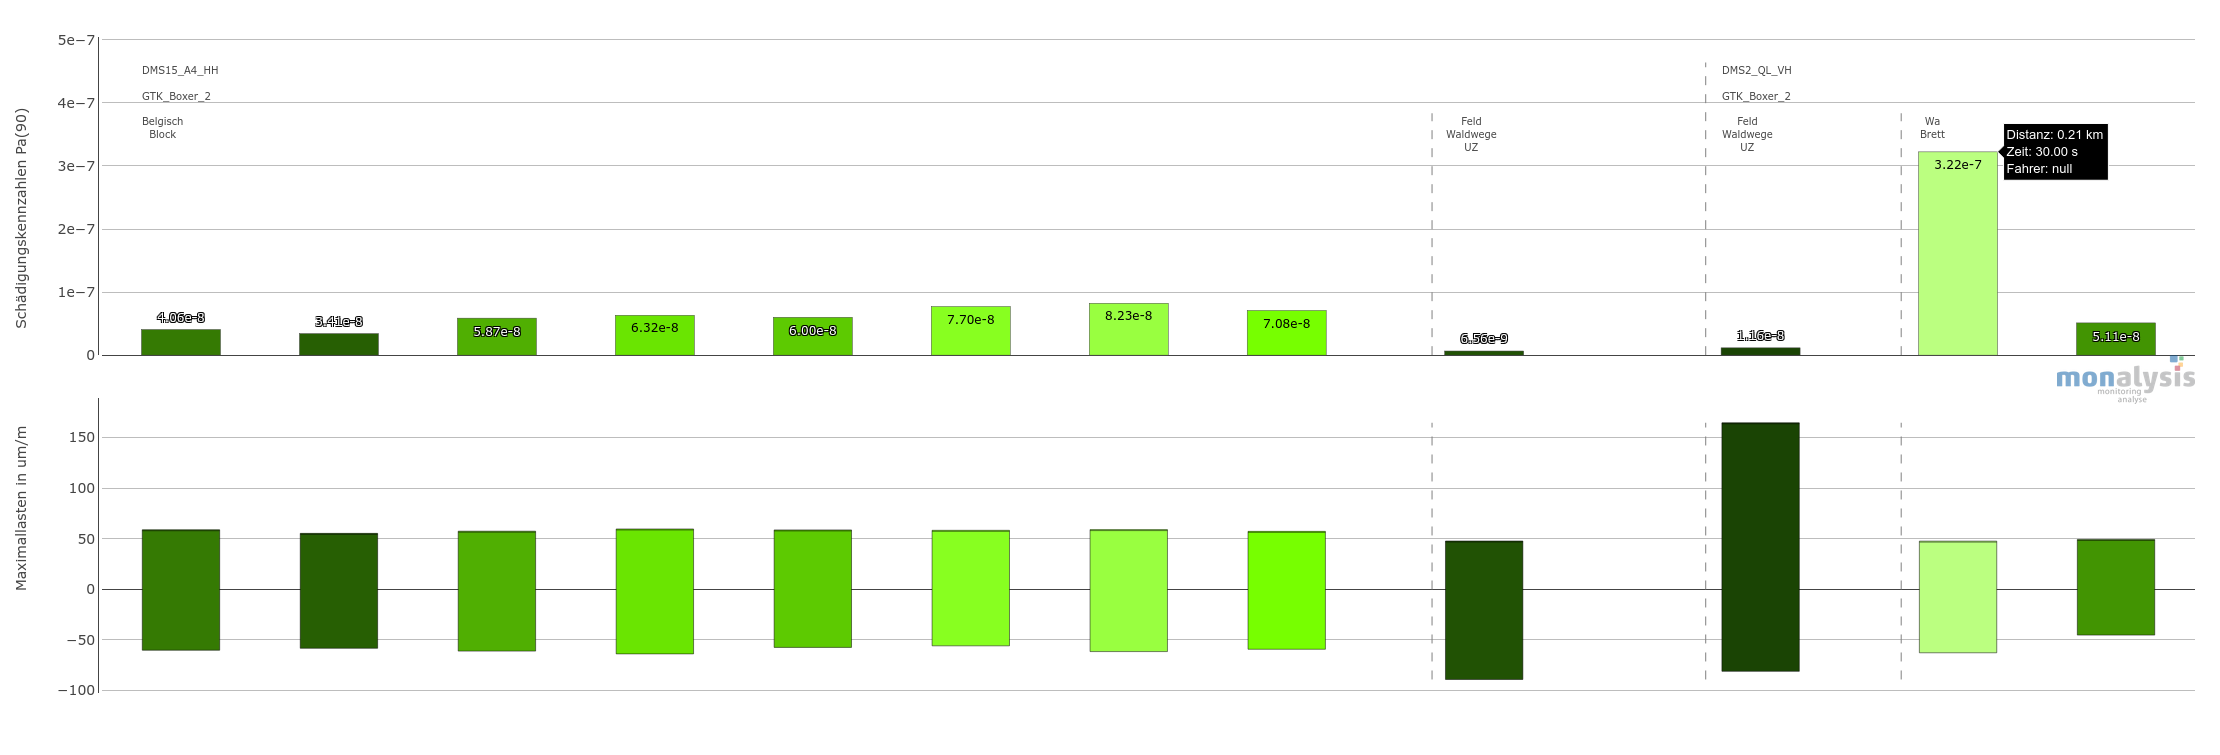
\includegraphics[width=1\linewidth]{gfx/top_vergleich_neu.png}
    \caption{Graph mit der kumulierten Schädigung im Vergleich mit Top-Filter}
    \label{fig:top_filter_vergleich}
\end{figure}
\noindent
Ein weiterer Graph, der ebenfalls bereits ohne Data-Storytelling existiert, sind die Zeitreihen. Diese werden in der alten Webseite nur als Linegraph dargestellt und wurden in dieser Arbeit durch die Trenderkennung erweitert. Dadurch können bei der Benutzung der Trenderkennung viele Erkenntnisse schnell und visuell ansprechend gewonnen werden. Werden die Graphen als Bilder exportiert, wird die Trenderkennung ebenfalls auf den exportierten Bildern dargestellt. In Abbildung \ref{fig:timeseries_compare} sind die beiden Zeitreihen-Darstellungen im direkten Vergleich zu sehen.\\
\begin{figure}[!h]
    \centering
    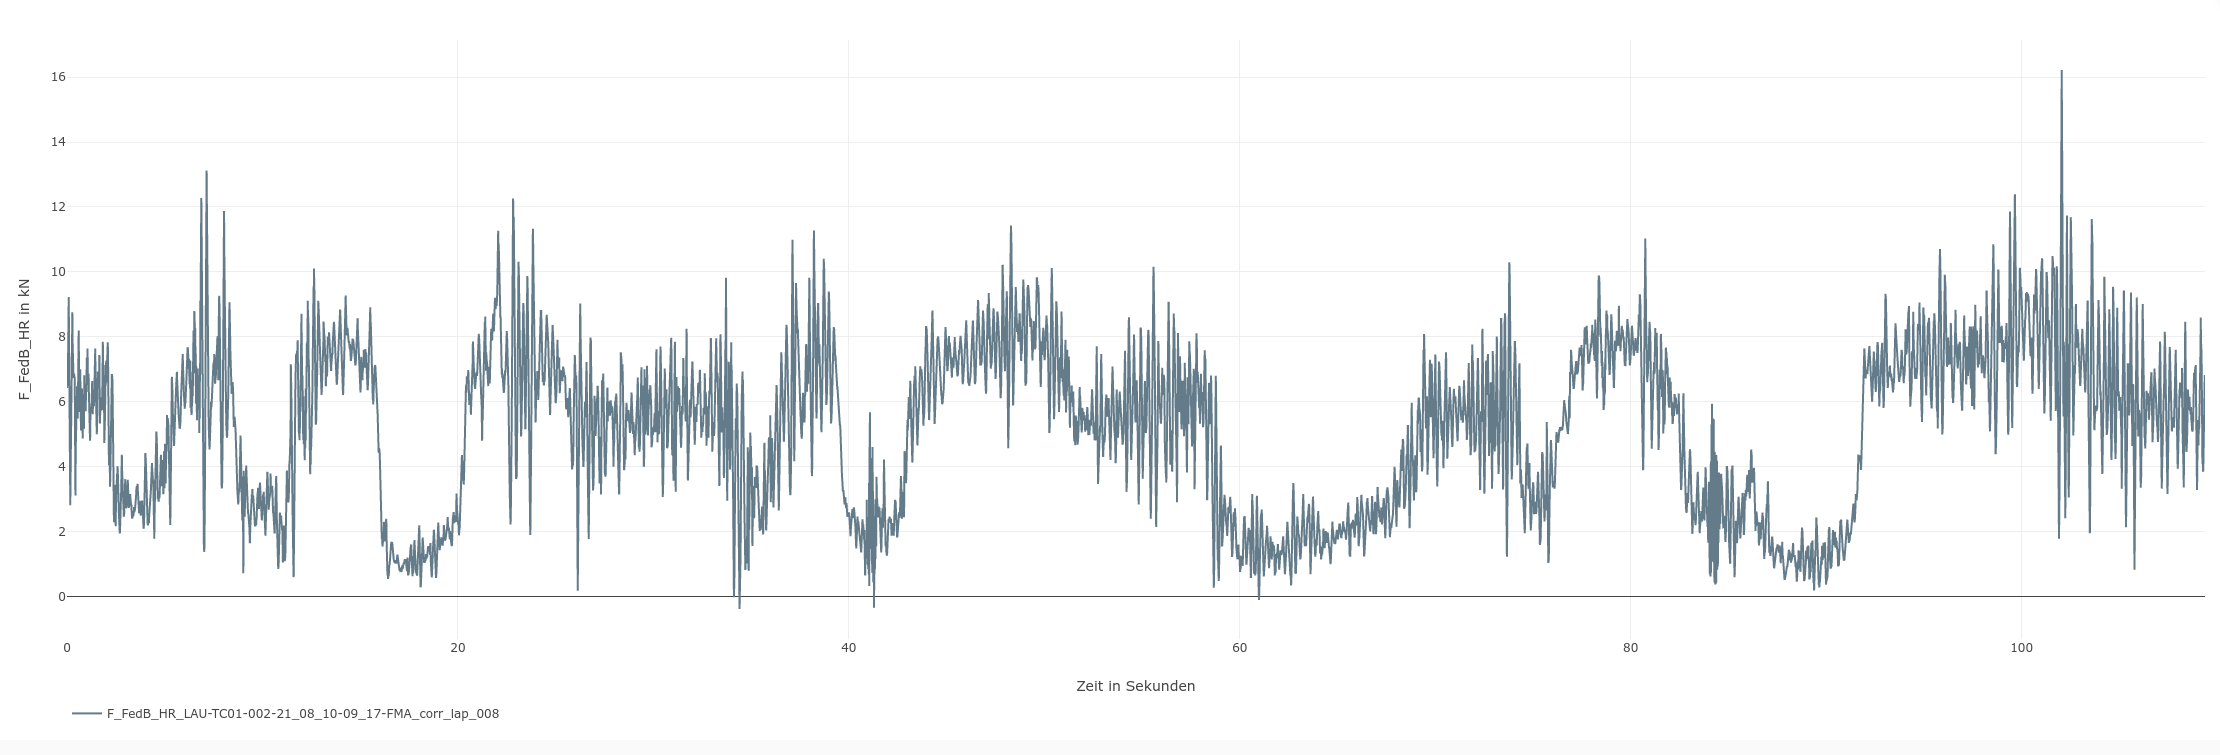
\includegraphics[width=1\linewidth]{gfx/timeseries_old.png}
    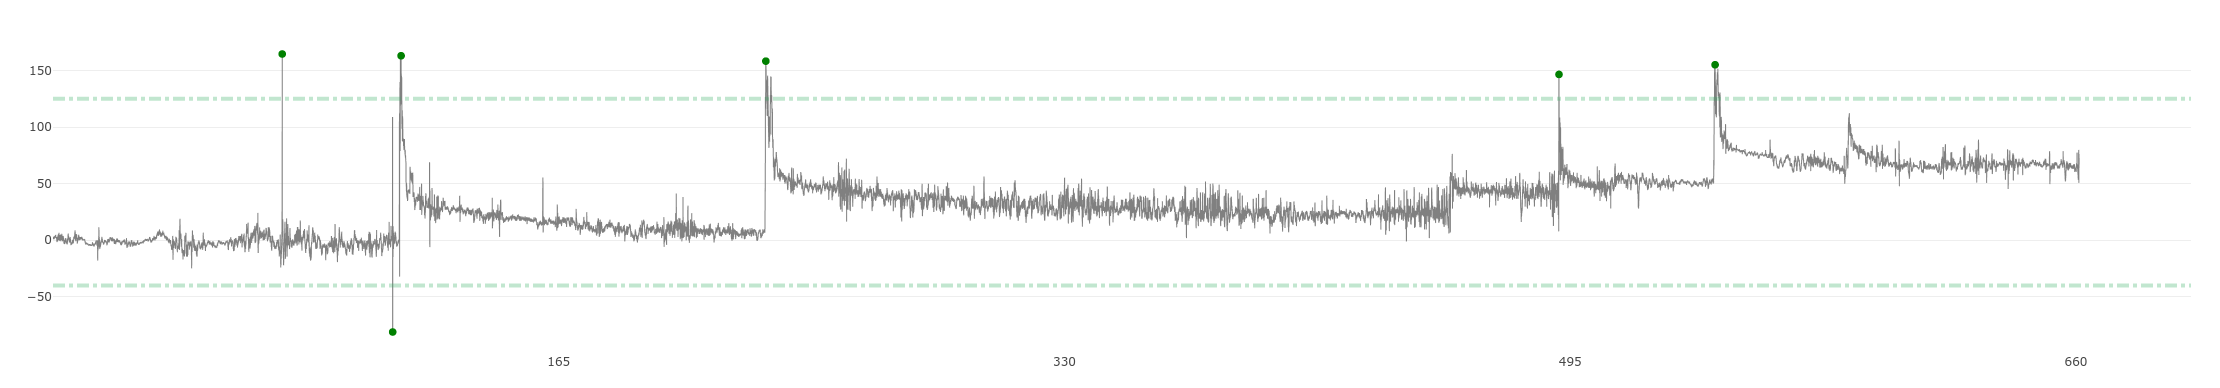
\includegraphics[width=1\linewidth]{gfx/timeseries_new.png}
    \caption{Zeitreihen im Vergleich}
    \label{fig:timeseries_compare}
\end{figure}
\noindent
Der letzte Graph, der bereits in einer Webseite existiert, sind die Fingerprints. Durch die Reduzierung der verschiedenen Elemente des Graphen konnte gleichzeitig ein deutlich geordneterer und informativerer Graph erstellt werden. In dem Graphen, der in dieser Arbeit erzeugt wurde, können anstatt einer alle drei Raumrichtungen dargestellt werden. Ebenso wird durch das Data-Storytelling direkt sichtbar, welcher Punkt im Graphen die Zahl Eins erreicht hat. Dadurch kann schneller erkannt werden, bei welcher Messung die kritische Leistung erreicht wurde. In Abbildung \ref{fig:fingerprints_compare} ist der Vergleich zu betrachten.\\\\ 
\begin{figure}[!h]
    \centering
    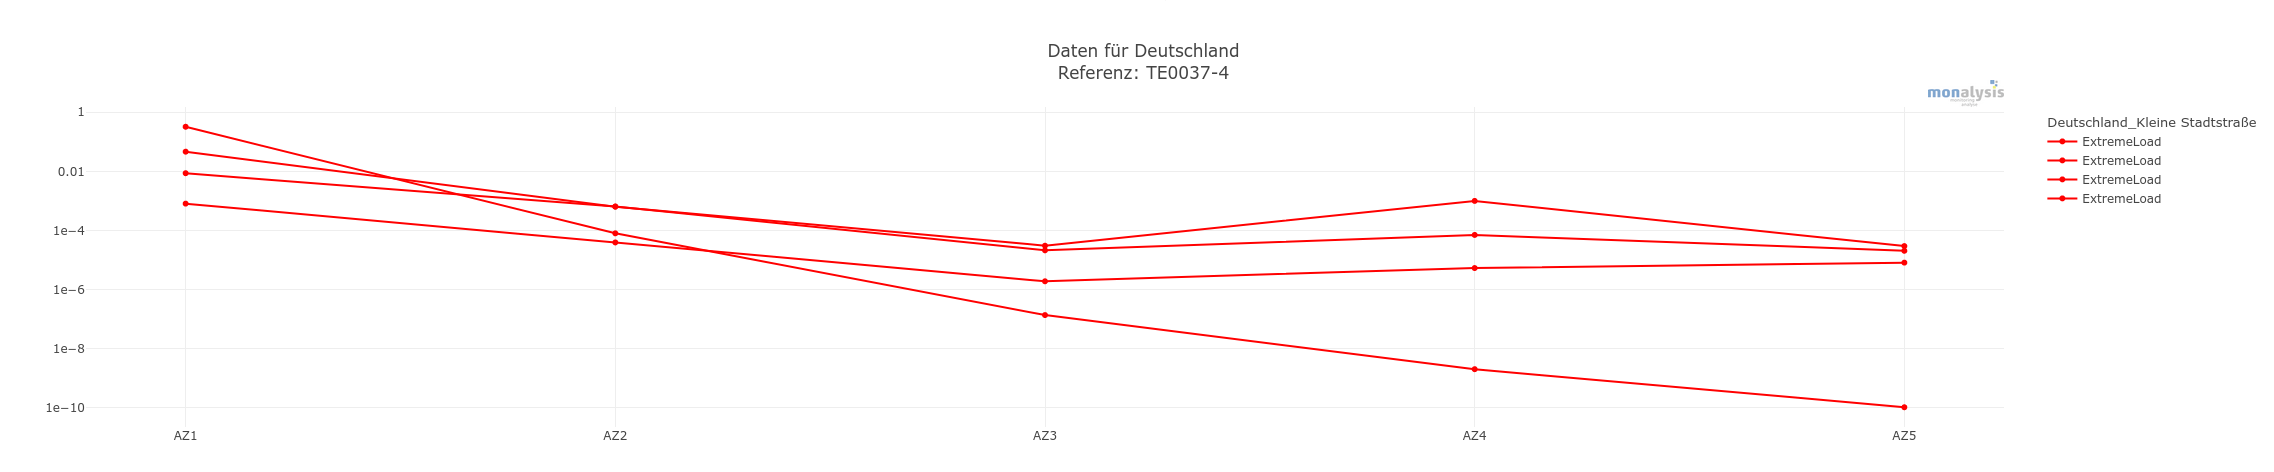
\includegraphics[width=1\linewidth]{gfx/fingerprints_old.png}
        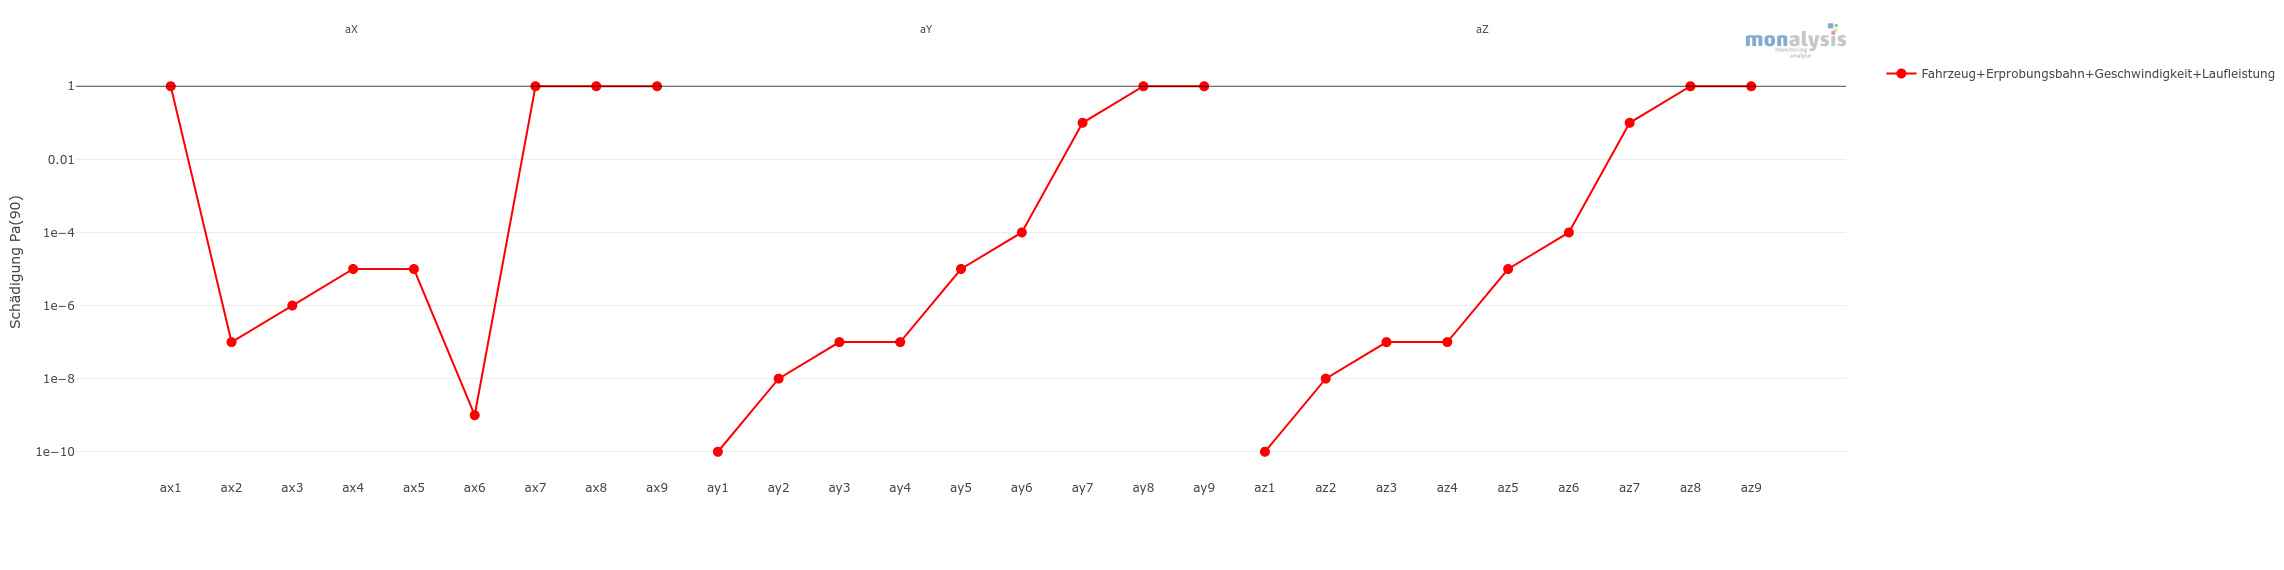
\includegraphics[width=1\linewidth]{gfx/fingerprints_new.png}
    \caption{Fingerprints im Vergleich}
    \label{fig:fingerprints_compare}
\end{figure}
\noindent
Durch diese Gegenüberstellungen lässt sich gut erkennen, dass das Data-Storytelling ein wertvolles Werkzeug ist, um Graphen informativ und Daten für den Benutzer verständlich darzustellen. Für Benutzer, die im Thema Betriebsfestigkeit und Fahrzeuge keine Experten sind, ist das Data-Storytelling wichtig, da sich durch den Einsatz des Storytellings lenken lässt, was der Benutzer als Erstes wahrnimmt.  
\section{Umfrage zu den Data-Storytelling-Graphen}
Zur Beurteilung des Data-Storytellings wurden die Experten aus dem Interview am Anfang der Arbeit zur Erkennung der Trends erneut interviewt. Dabei ist das Interview mit Jeele Böggemann in Anhang \ref{appendix:interview_ende_boeggemann}, das Interview mit Benedikt Mundl in Anhang \ref{appendix:interview_ende_mundl}, das Interview mit Michael Städele in Anhang \ref{appendix:interview_ende_staedele} und das Interview mit Florian Zenzinger in Anhang \ref{appendix:interview_ende_zenzinger} zu finden. Ihnen wurden die Graphen aus der entwickelten Webseite gezeigt sowie Fragen aus dem Interviewleitfaden in Anhang \ref{appendix:interview_ende} gestellt. Zur Auswertung der Interviews wurde erneut nach den Methoden von \cite{Mayring.2022}, \cite{Kuckartz.2022} und \cite{AndreMorgensternEinenkel.2023} eine inhaltlich strukturierende qualitative Inhaltsanalyse erstellt. Insgesamt sind sich die Experten einig, dass das Data-Storytelling eine deutliche Verbesserung der Graphen sowohl visuell, im Sinne des einfacheren Verstehens, als auch in der Geschwindigkeit, mit der die Graphen analysiert werden können, erreicht hat. Zu der Geschwindigkeit der Analyse mit Data-Storytelling äußern sich Jeele Böggemann in den Zeilen \lref{appendix:interview_ende_boeggemann:schneller}--770 und \lref{appendix:interview_ende_boeggemann:schneller_2}--786, Benedikt Mundl in den Zeilen \lref{appendix:interview_ende_mundl:geschwindigkeit}--839, Michael Städele in den Zeilen \lref{appendix:interview_ende_staedele:schneller}--926 und \lref{appendix:interview_ende_staedele:schneller_2}--941 sowie Florian Zenzinger in den Zeilen \lref{appendix:interview_ende_zenzinger:schneller}--992 und \lref{appendix:interview_ende_zenzinger:schneller_2}--1002. Alle vier Experten sind sich einig, dass die Analysen schneller durchgeführt werden können. Zu der Vereinfachung der Analyse der Graphen erklären Benedikt Mundl (Zeilen \lref{appendix:interview_ende_mundl:leichter}--862) und Michael Städele (Zeilen \lref{appendix:interview_ende_staedele:leichter}--933), dass es besonders bei Benutzern, die noch wenig versiert mit den Daten umgehen können, eine große Hilfe ist, Data-Storytelling zu benutzen. Dieser Aussage stimmt auch Florian Zenzinger in der Zeile \lref{appendix:interview_ende_zenzinger:leichter} zu, wobei er anmerkt, dass die Graphen „deutlich übersichtlicher“ seien.\\ Zudem stimmen alle Experten überein, dass das Data-Storytelling auch in Zukunft auf weitere fahrzeugbasierte Daten angewandt werden soll beziehungsweise in bereits vorhandenen Projekten nachträglich implementiert werden soll (Jeele Böggemann: Zeile \lref{appendix:interview_ende_boeggemann:neue}, Michael Städele: Zeilen \lref{appendix:interview_ende_staedele:neue}--920, Benedikt Mundl: Zeilen \lref{appendix:interview_ende_mundl:neue}--833, Florian Zenzinger: Zeile \lref{appendix:interview_ende_zenzinger:neue}). Als Nachteil wird von dem Experten Benedikt Mundl (Zeilen \lref{appendix:interview_ende_mundl:nachteil}--876) die Schwierigkeit beim Finden von verständlichen Umschreibungen für manche Funktionen der Trenderkennung erwähnt. Dieser Nachteil wird mit der Einführung von Beispielen in dem Trenderkennungsmenü ausgeglichen. Von Michael Städele (Zeilen \lref{appendix:interview_ende_staedele:nachteile}--954) wird als Nachteil genannt, dass bei der Erkennung von Trends ein gewisser Konfigurationsaufwand entsteht, besonders bei den Einstellungen der Trenderkennung. Die Vorteile des Data-Storytellings werden von Michael Städele (Zeilen \lref{appendix:interview_ende_staedele:story}--910 und \lref{appendix:interview_ende_staedele:story_2}--941) zusammengefasst als „schnellere Möglichkeit, damit zu arbeiten“ und als „Fokussierung auf die wichtigen Werte“. Diese Vorteile werden auch von Benedikt Mundl (Zeilen \lref{appendix:interview_ende_mundl:story}--862) genannt. Insgesamt sind alle Experten der Meinung, dass das Data-Storytelling in dieser Arbeit erfolgreich war.
\section{Fazit}
Das Ziel dieser Arbeit war festzustellen, ob das Data-Storytelling einen Mehrwert für komplexe fahrzeugbasierte Daten bieten kann.
Zunächst wurde der Prozess des Data-Storytellings genauer analysiert, und im Anschluss wurden mehrere Experteninterviews durchgeführt, um die passenden Informationen zu identifizieren. Da es sich bei dem letzten Punkt des Data-Storytellings um das Erzählen einer Geschichte handelt, ist es wichtig zu verstehen, weshalb welche Informationen in den Daten von Bedeutung sind. Anhand der Ergebnisse des Experteninterviews wurde eine Trenderkennung implementiert, die dazu genutzt werden kann, verschiedene interessante Punkte in den Daten, wie minimale oder maximale Punkte, sowie verschiedene über längere Zeit anhaltende Verhalten zu charakterisieren. Anhand der Ergebnisse der Trenderkennung können mit dem Data-Storytelling Geschichten entwickelt werden. Zudem wurde in dieser Arbeit der Prozess des Data-Storytellings an mehreren Graphen angewendet und je nach Ziel des Graphen angepasst. Diese Graphen konnten mit bereits existierenden Graphen, die einem ähnlichen Zweck dienen, verglichen werden. Hierdurch ist klar zu erkennen, dass die Graphen, die durch den Data-Storytelling-Prozess aufbereitet wurden, leichter zu verstehen sind und schneller entscheidende Inhalte der Visualisierung zu erkennen sind. Diese These wurde von den bereits am Anfang interviewten Experten bestätigt. Von den Experten wurde auch klar formuliert, dass sich das Data-Storytelling gut für fahrzeugbasierte Daten eignet und weiterhin auf diese Daten angewendet werden soll. Obwohl das Data-Storytelling für einige Graphen eine große Bereicherung ist, kann es für einige Anwendungsfälle schwierig sein, die passende Geschichte oder den passenden Call-To-Action zu definieren. Dabei ist hauptsächlich zu beachten, ob der Graph zu reinen Beobachtung von Daten genutzt werden soll, oder ob tatsächlich eine Aussage aus den Daten hervorgeht. Trotzdem kann man mit den ersten drei Schritten des Prozesses des Data-Storytelling nahezu jeden Graphen verbessern. Auch ist aus dieser Arbeit hervorgegangen, dass die Art der Daten, die beim Data-Storytelling dargestellt werden, eine sehr große Rolle spielen. Die Erstellung der Graphen ist sehr individuell, was besonders beim Erzählen der Geschichte aufgefallen ist. Deswegen wäre es interessant, das Data-Storytelling in Zukunft auch auf andere Daten angewendet zu sehen, besonders da jeder Anwendungsfall einzigartig ist. 